\documentclass{article}

% Language setting
% Replace `english' with e.g. `spanish' to change the document language
\usepackage[english]{babel}

% Set page size and margins
% Replace `letterpaper' with `a4paper' for UK/EU standard size
\usepackage[letterpaper,top=2cm,bottom=2cm,left=3cm,right=3cm,marginparwidth=1.75cm]{geometry}

% Useful packages
\usepackage{amsmath}
\usepackage{graphicx}
\usepackage[colorlinks=true, allcolors=blue]{hyperref}
\usepackage{caption}
\usepackage{subcaption}
\usepackage{lipsum} 

\title{Plenoxels and extension to point clouds}
\author{Nissim Maruani}

\begin{document}
\maketitle


\begin{figure}[!h]
 \centering
\begin{subfigure}{.19\textwidth}
  \centering
  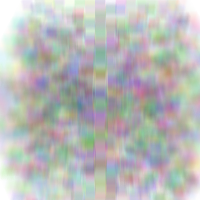
\includegraphics[width=\linewidth]{figs/model0.png}  
\end{subfigure}
\begin{subfigure}{.19\textwidth}
  \centering
  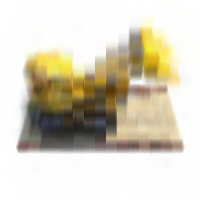
\includegraphics[width=\linewidth]{figs/model1.png}  
\end{subfigure}
\begin{subfigure}{.19\textwidth}
  \centering
  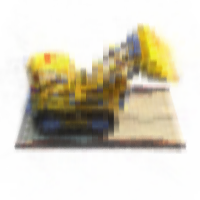
\includegraphics[width=\linewidth]{figs/model3.png}  
\end{subfigure}
\begin{subfigure}{.19\textwidth}
  \centering
  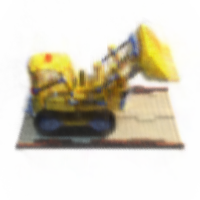
\includegraphics[width=\linewidth]{figs/model15.png}  
\end{subfigure}
\begin{subfigure}{.19\textwidth}
  \centering
  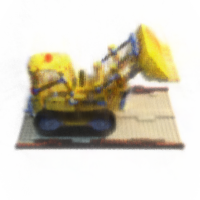
\includegraphics[width=\linewidth]{figs/model32.png}  
\end{subfigure}
     \caption{Our model at epoch {0, 2, 6, 14, 22}. Total computation time: 35 minutes on a single GPU.}
    \label{fig:lego_optim}
\end{figure}


\begin{abstract}
\lipsum[0-1] TODO
\cite{plenoxels}
\cite{nerf}
\cite{spacecarving}
\cite{directvoxgo}
\cite{instant}
\end{abstract}


\section{Introduction}

The most straightforward way to capture 3D objects from the real world is to use special sensors such as the Kinect or more expensive scanning devices. Another approach relies solely on RGB images: by combining photographs taken at several known viewpoints, one is able to render novel views of a scene. A year ago, a method known as \textit{NeRF} (for Neural Radiance Field \cite{nerf}) tackled this challenge by using a deep neural network to simultaneously shapes and shadings. More recently, a new approach known as \textit{Plenoxels} \cite{plenoxels} showed that directly optimizing a voxel grid allowed better results with faster computations. This project is focused on this paper. We re-implemented parts of it and TODO.
\footnote{\url{https://github.com/nissmar/Radiance-Fields}}

\section{Our implementation}

\subsection{Given code}


The given code associated to the plenoxels paper requires the compilation of a custom CUDA extension which parallelizes operations. Unfortunately, it requires a CuDNN developer account and quite a bit of C++ experience. In order to avoid losing time on hazardous compilations, we decided to ignore the given code and re-implement everything \textbf{from scratch}, except for the utilities functions \textit{get\_data} and \textit{get\_rays\_np} (30 lines of code) from the original plenoxels repository \footnote{\url{https://github.com/sarafridov/plenoxels}} and the Python file \textit{ply.py}, given in the TP of this course.  

\subsection{Our implementation}


Since our implementation is "homemade", it doesn't contain every extension described in the paper. It is slower (because it doesn't use a custom CUDA kernel) but still usable in finite time: a simple 128x128x128 grid can be trained in 30 minutes. 

%Our code is organized in the following manner:
%\begin{itemize}
%\item The file \textit{VoxelGrid.py} contains the different voxel grids (RGB colors, spherical harmonics and tri-linear interpolation) 
%\item The files \textit{main.py} and \textit{main\_spherical.py} are used to optimize our grids
%\item The different jupyter notebooks allow for a more interactive training and computation of PSNR
%\item Some useful functions (including \textit{get\_data} and \textit{get\_rays\_np}) are located inside \textit{utilities.py}.
%\end{itemize}

The Plenoxel paper introduces remarkable concepts and the given implementation is no less great: the custom CUDA kernel parrelize across rays, which allow a different number of active voxel for each ray and much faster computations. Reproducing the results was a challenge, and improving the given method (in terms of speed or quality of results) was impossible in the scope of this project. TODO dernière approche.
% However, we found a way to extend this approach by integrating a point cloud export to the code, which links this project to the NPM3D course.   

\subsection{Datasets}

\begin{figure}[!h]
 \centering

\begin{subfigure}{.24\textwidth}
  \centering
  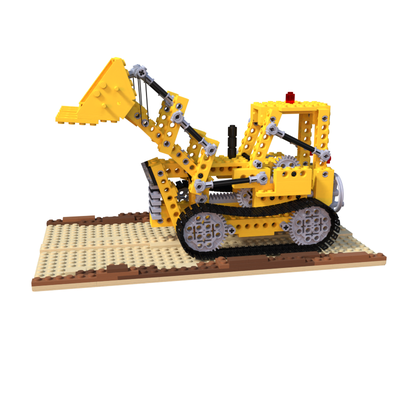
\includegraphics[width=\linewidth]{figs/results/lego_ref.png}  
\end{subfigure}
\begin{subfigure}{.24\textwidth}
  \centering
  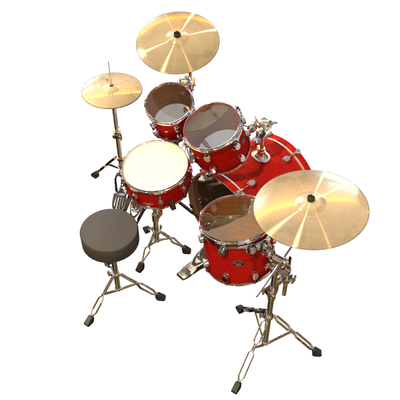
\includegraphics[width=\linewidth]{figs/results/drums_ref.png}  
\end{subfigure}
\begin{subfigure}{.24\textwidth}
  \centering
  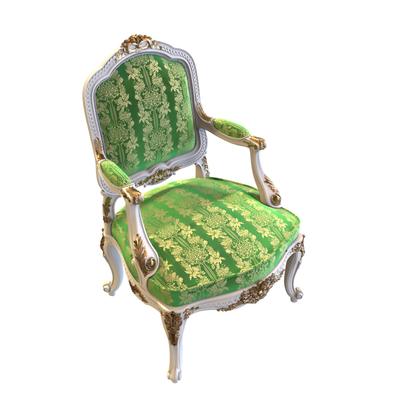
\includegraphics[width=\linewidth]{figs/results/chair_ref.png}  
\end{subfigure}
\begin{subfigure}{.24\textwidth}
  \centering
  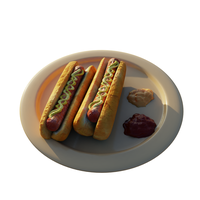
\includegraphics[width=\linewidth]{figs/results/hotdog_ref.png}  
\end{subfigure}


\begin{subfigure}{.24\textwidth}
  \centering
  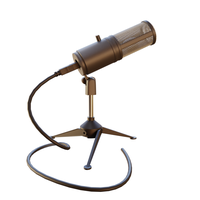
\includegraphics[width=\linewidth]{figs/results/mic_ref.png}  
\end{subfigure}
\begin{subfigure}{.24\textwidth}
  \centering
  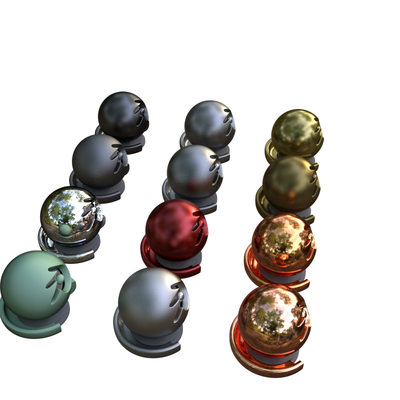
\includegraphics[width=\linewidth]{figs/results/materials_ref.png}  
\end{subfigure}
\begin{subfigure}{.24\textwidth}
  \centering
  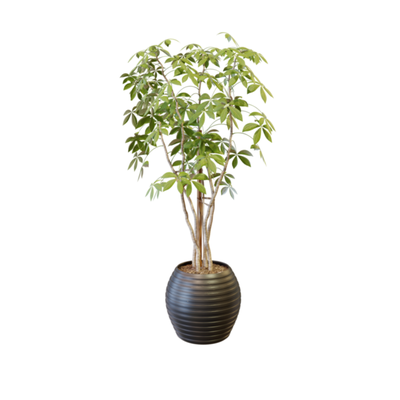
\includegraphics[width=\linewidth]{figs/results/ficus_ref.png}  
\end{subfigure}
\begin{subfigure}{.24\textwidth}
  \centering
  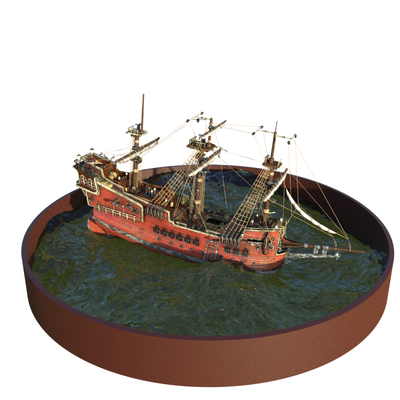
\includegraphics[width=\linewidth]{figs/results/ship_ref.png}  
\end{subfigure}

     \caption{Test images from the \textit{nerf\_synthetic} datasets}
    \label{fig:dataset}
\end{figure}


We used the \textit{nerf\_synthetic} dataset, composed of 8 virtual objects.
\section{Related works}



\subsection{Classical methods}

Before the rise of neural networks, some methods already existed to render novel views from images: one of them is called \textit{Space Carving} \cite{spacecarving}. Starting from a dense grid, the voxels from the surface are removed one by one if they aren't consistent with every photograph. This (quite slow) method successfully captures the 3D shape and texture of the photographed scenes, but is unable to capture the transparent/specular properties of the objects. However, we noticed the rigor of the authors who provide theoretical guarantees, absent from nowadays' optimization methods.

\subsection{NeRF rendering}

The \textit{NeRF} \cite{nerf} approach consists of training a fully-connected network which takes a 5D input $(x,y,z,\theta,\phi)$ composed of a 3D position and a viewing direction, and outputs a 4D tensor $(r, g, b, \sigma)$ composed of an RGB color and an opacity $\sigma$. For each pixel of the rendered image, $N$ points are sampled along a camera ray and their colors and intensities are integrated to obtain a final $RGB$ value. This method achieved state-of-the-art when it was published, as it allowed to reproduce shading and specular effects efficiently. The training time, however, was quite slow (12 hours for a single scene).

\subsection{Concurrent papers and posterior approach}

\textit{DirectVoxGo} \cite{directvoxgo} is similar to Plenoxels: the main differences are that it uses a neural network (and not a custom CUDA implementation). It produces NeRF-comparable results in less than 15 minutes. More recently, a method using multiresolution Hash encoding \cite{instant} was able to reproduce the same results in less than 1 second!

\section{The method}

In this section, we'll describe the method of the original paper \cite{plenoxels}, and list the different between their implementation (see Figure \ref{fig:plenoxel}) and ours.



\begin{figure}[!h]
\centering
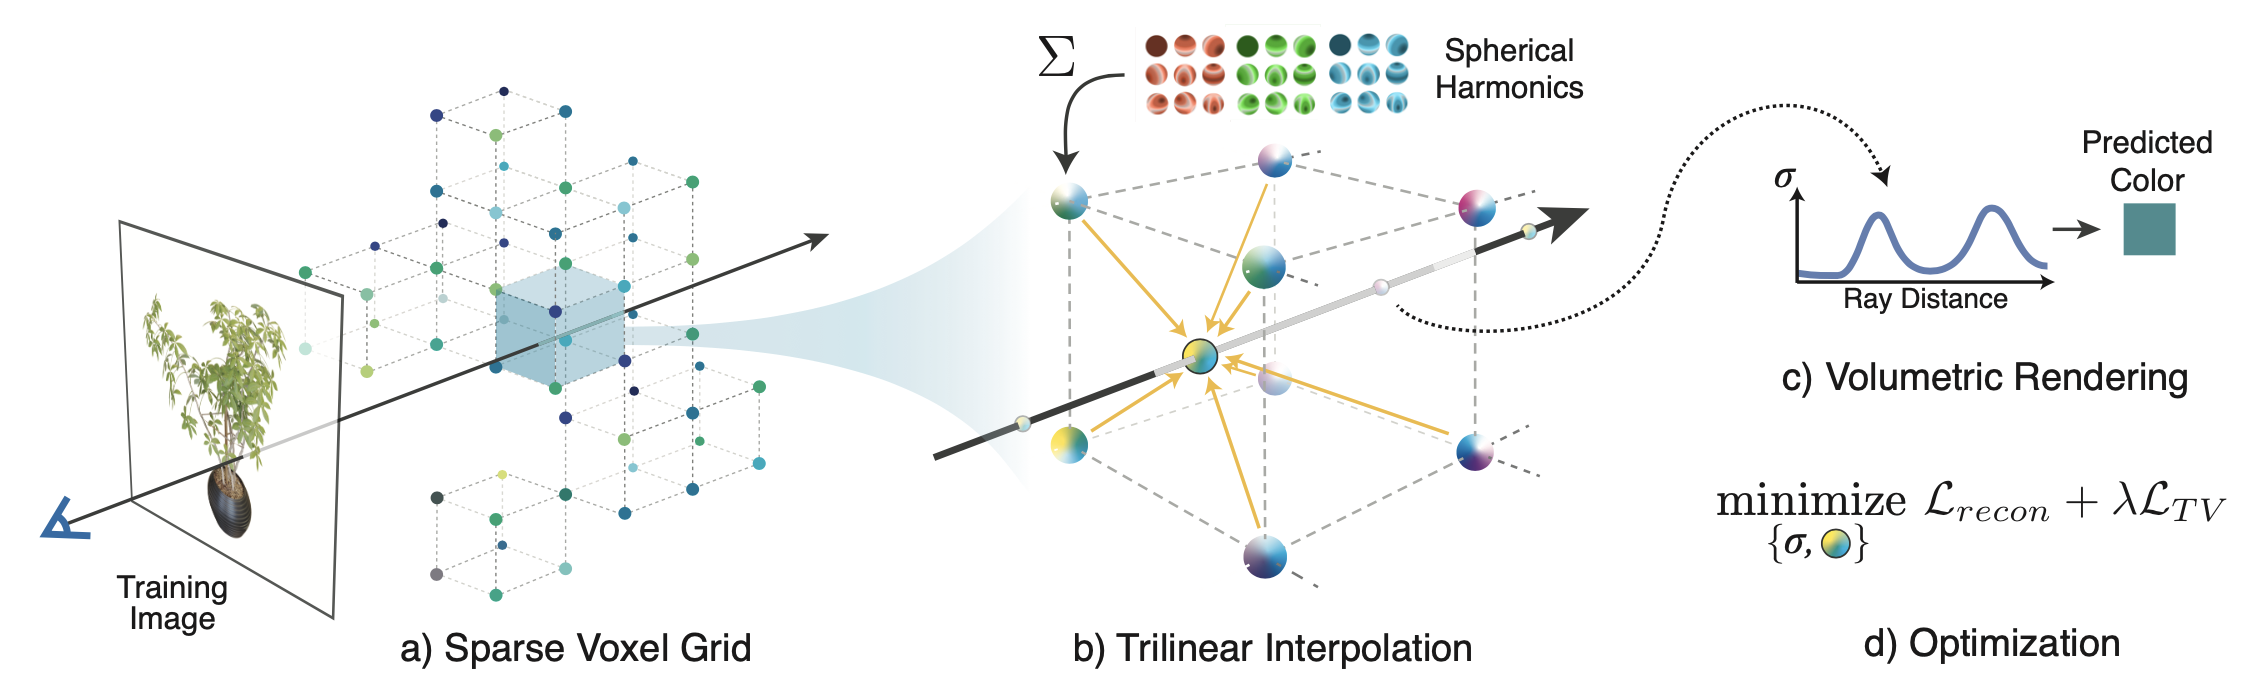
\includegraphics[width=1.\textwidth]{figs/plen_pipeline.png}
\caption{\label{fig:plenoxel} [image source: \cite{plenoxels}] The plenoxels method is composed of four steps : (a) camera rays are extracted from training images and sampled on a sparse voxel grid ; (b) the spherical harmonics of degree 9 and opacities are computed for each sample through trilinear interpolation ; (c) the resulting colors and opacities are summed to obtain a single pixel value for each ray (d) the mean squared error loss with a total variation regularizer is back-propagated to optimize the grid}
\end{figure}



\subsection{The voxel grid}

The clever idea of Plenoxels is to optimize a voxel grid directly. Each voxel stores an opacity $\sigma \in \mathbf{R}^+$ along with spherical harmonics coefficients in $[0,1]$. These spherical harmonics allow each voxel to have a different color depending on the viewing direction, which renders specular effects and reflections.

The original paper uses a sparse voxel grid optimized with the custom CUDA implementation. Ours is a dense voxel grid which which justifies the lower definition (128x128x128 vs 512x512x512) and the longer computation time. We experimented with spherical harmonics of degree 1 (each voxel has a single color)
and 4, but we couldn't get good results with the latter. It may be due to the more complicated convergence. 

\subsection{Color estimation from camera rays}

Once this grid is initialized at random, we optimize its voxels based on images taken from known viewpoints. Each pixel $p_x$ of the training images corresponds to a certain camera ray $r(p_x) \in (\mathbf{R}^3, \mathbf{R}^3)$ composed of an origin and a direction. We sample this ray with $N=200$ points, compute the points colors and opacities via nearest neighbour interpolation (we implemented trilinear interpolation like in the paper but it was 8 times slower) and sum the sampled points to obtain the estimated RGB color $\hat{c}(r(p_x))$:
\[\hat{c}(r(p_x)) = \sum_{0\leq i<N} T_i (1 - \exp(-\sigma_i \delta_i)) c_i\] 

Where $ T_i = \exp(- \sum_{0\leq j<i} \sigma_j \delta_j)$ represents how much light is transmitted to sample $i$ and $\delta_i$ represents the distance between samples.\\ 

At first, we were quite puzzled at by this formula, so we considered the following example: an object of constant color $c$ and opacity $\sigma$ sampled by $N$ points. The distance between points is thus $D/N$, where $D$ is a constant. The resulting color of a ray through this material is:
\[ \sum_{1 \leq i \leq N} \exp(- (i-1)\frac{ \sigma D}{N})(1 - \exp(-  \frac{ \sigma D}{N}))c = c (1 - exp(- \sigma D))\]

In this simple case, the color is indeed independent from the number of samples. Note that it assumes however constant values of color and opacity between samples.


\subsection{Optimization}
The loss is then computed as $L = \sum_{p_x} \|p_x -\hat{c}(r(p_x)) \|^2 + \lambda_{TV}  L_{TV}$, and back-propagate through the grid. At each training step, we sample 5000 random rays and compute the total variation over the whole grid. We used an SGD optimizer to do the gradient descent with a learning rate of 1000, and $\lambda_{TV} = 10^{-4}$. 

\section{Results and experiments}

\subsection{Visual interpretation}


\begin{figure}[!h]
 \centering

\begin{subfigure}{.24\textwidth}
  \centering
  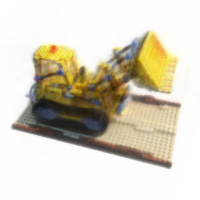
\includegraphics[width=\linewidth]{figs/results/lego.png}  
\end{subfigure}
\begin{subfigure}{.24\textwidth}
  \centering
  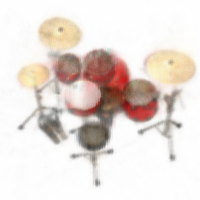
\includegraphics[width=\linewidth]{figs/results/drums.png}  
\end{subfigure}
\begin{subfigure}{.24\textwidth}
  \centering
  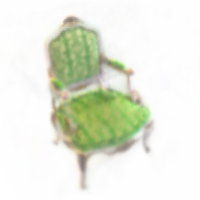
\includegraphics[width=\linewidth]{figs/results/chair.png}  
\end{subfigure}
\begin{subfigure}{.24\textwidth}
  \centering
  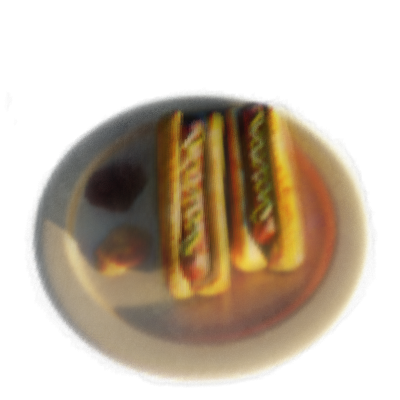
\includegraphics[width=\linewidth]{figs/results/hotdog.png}  
\end{subfigure}


\begin{subfigure}{.24\textwidth}
  \centering
  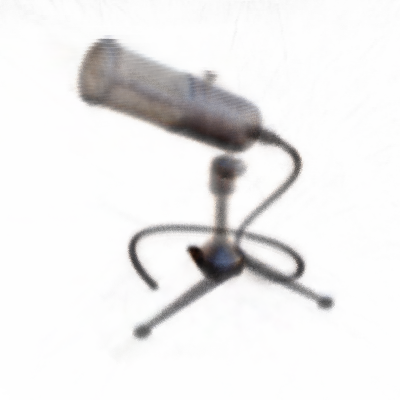
\includegraphics[width=\linewidth]{figs/results/mic.png}  
\end{subfigure}
\begin{subfigure}{.24\textwidth}
  \centering
  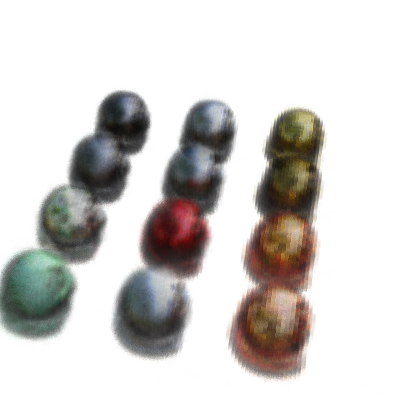
\includegraphics[width=\linewidth]{figs/results/materials.png}  
\end{subfigure}
\begin{subfigure}{.24\textwidth}
  \centering
  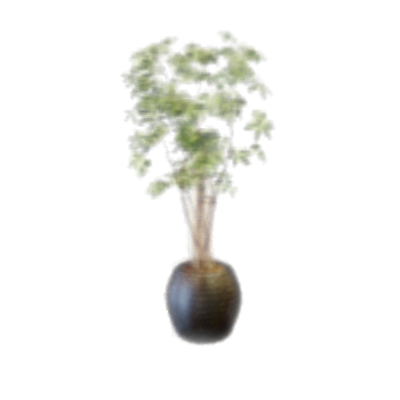
\includegraphics[width=\linewidth]{figs/results/ficus.png}  
\end{subfigure}
\begin{subfigure}{.24\textwidth}
  \centering
  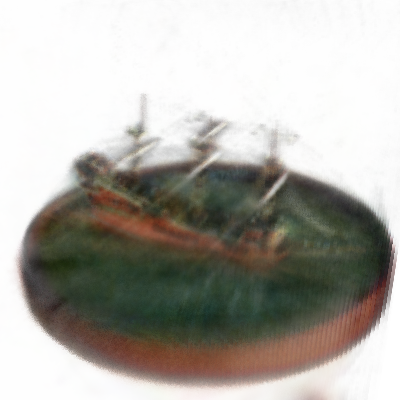
\includegraphics[width=\linewidth]{figs/results/ship.png}  
\end{subfigure}

     \caption{Our models evaluated on novel viewpoints (see our GitHub repository for animated GIFs)}
    \label{fig:results}
\end{figure}

Considering the fact that we couldn't use a custom CUDA kernel, we are quite satisfied with our results. They are visually plausible, enven though at slight blur is sometimes noticeable. As we use spherical harmonics of degree 1, specular effects aren't rendered, and perhaps that is why some surfaces are semi-transparent. Visually, the ship is the least realistic: because of its small details, a grid of size 128x128x128 isn't sufficient to represent it.

\subsection{PSNR comparison}

The PSNR (for peak signal to noise ratio), defined as $PSNR = 10\log_{10}(1/MSE)$, is an image metric often used in image restoration. In this context, novel test views are used to compare the rendered model and the real image. In the original paper, a score of $23.74$ dB is reached with a 128x128x128 grid and nearest neighbor interpolation. We obtain a score of $TODO$. TODO PSNR We are quite satisfied with this result, considering the fact that we don't use spherical harmonics. 

\begin{table}[!h]
\centering
\begin{tabular}{|l||c|r|}
\hline
Dataset & TV (30 min training) & No TV (30 min training) \\\hline
Drums & 20.12 dB & 20.12 dB \\
Chair & 23.69 dB & 23.70 dB \\ 
Ship & 20.65  dB & 20.66 dB\\
Ficus & 23.86 dB & 23.85 dB\\
HotDog &  23.79 dB &  23.75 dB  \\
Materials &  20.98 dB &  20.99 dB \\
Lego &   21.43 dB &  21.42 dB  \\
Mic &  22.32 dB & 22.29 dB \\

\hline \hline
Mean & 22.10 ± 1.4  dB & 22.10 ± 1.4 dB \\
\hline 
\end{tabular}
\caption{\label{tab:psnr}PSNR on different training methods.}
\end{table}

\subsection{Adaptative grid size for faster optimization}


\begin{figure}[!h]
\centering
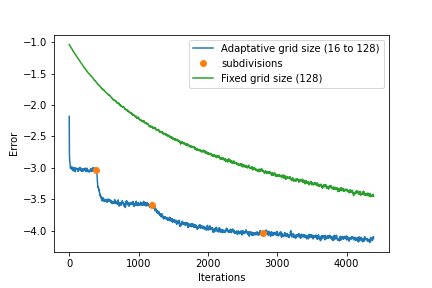
\includegraphics[width=0.5\textwidth]{figs/training_mic.png}
\caption{\label{fig:subd} Evolution of the error curve on the microphone model}
\end{figure}

In the paper, they subdivide the voxel grid via tri-linear interpolation to boost the training phase. We tested and implemented this method which greatly accelerated our optimization (Figures \ref{fig:lego_optim} and \ref{fig:subd}). We use grids of size ${16, 32, 64, 128}$, on respectively ${2, 4, 8, 8}$ epochs with a learning rate of ${1000, 1000, 500, 500}$. We use trilinear interpolation on colors and opacities to subdivide the grid.


\section{Using plenoxels to generate point clouds}

\subsection{CloudCompare pipeline}

A point cloud can be seen as a voxel grid with discrete (0 or 1) opacities. We implemented a \textit{.ply} export of our voxel grids, storing the RGB colors and the opacity as a scalar field. 

The point cloud is then loaded in CloudCompare. We found that applying the following transformations resulted in a clean, usable point cloud:

\begin{itemize}
\item \textbf{Edit $>$ Scalar fields $>$ Filter by value} (Range $2.0; +\infty$) to remove the transparent voxels
\item \textbf{Tools $>$ Clean $>$ Noise filter} (Radius $0.01$) to clean the point cloud
\item \textbf{Tools $>$ Clean $>$ S.O.R. filter} (Radius $0.2$) to remove the outliers.
\end{itemize}



\begin{figure}[!h]
 \centering
\begin{subfigure}{.25\textwidth}
  \centering
  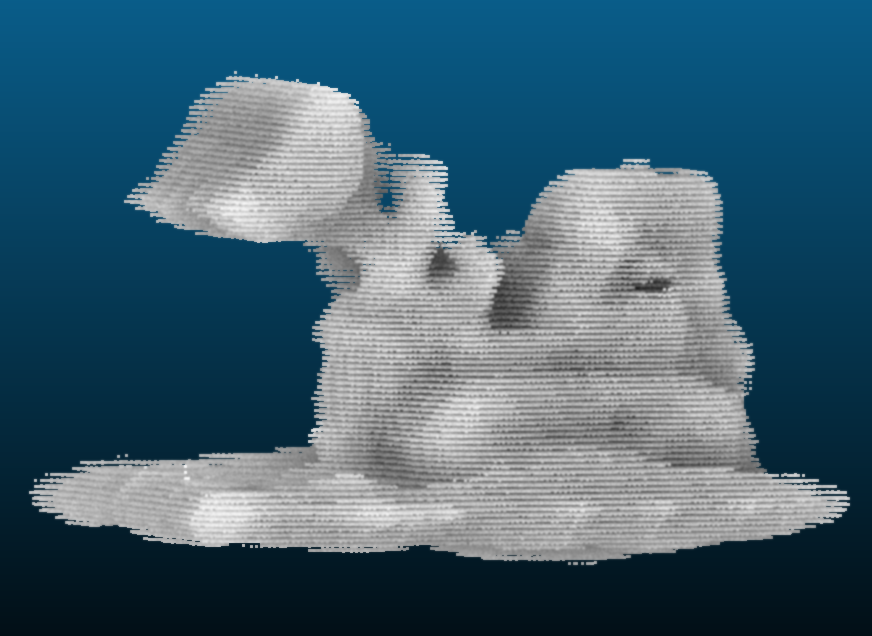
\includegraphics[width=\linewidth]{figs/lego_pc_no.png}  
\end{subfigure}
\begin{subfigure}{.25\textwidth}
  \centering
  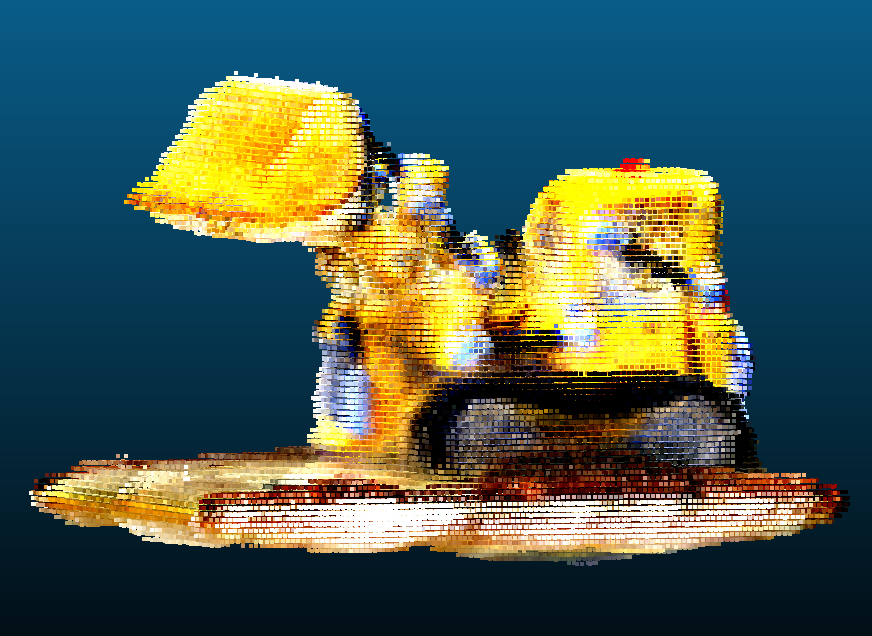
\includegraphics[width=\linewidth]{figs/lego_pc.png}  
\end{subfigure}
\begin{subfigure}{.21\textwidth}
  \centering
  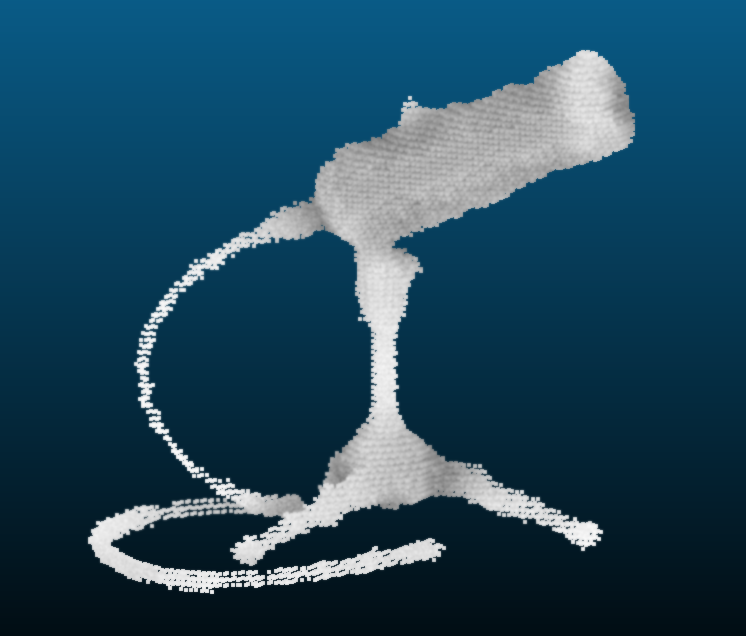
\includegraphics[width=\linewidth]{figs/mic_pc_no.png}  
\end{subfigure}
\begin{subfigure}{.21\textwidth}
  \centering
  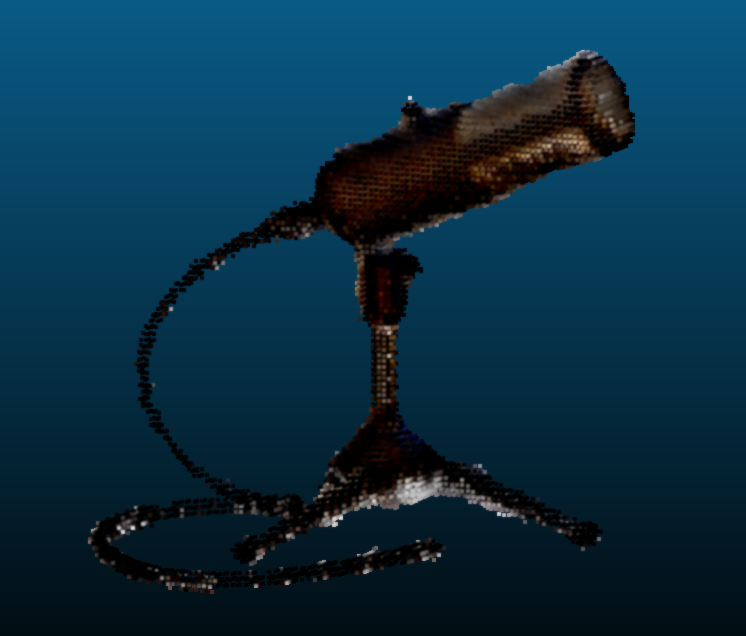
\includegraphics[width=\linewidth]{figs/mic_pc.png}  
\end{subfigure}
     \caption{Lego and mic models loaded in cloud compare}
    \label{fig:cc}
\end{figure}

 
\subsection{Discussion}

Although these parameters work great, the optimal ones may vary for each model (little less value filter for the lego model, little more noise filter for the hotdog model..). We are pretty satisfied with the results, and a good extension to this project would be to compare the point cloud obtained with this method and a more specialized device (kinect...) on a real scene.

\section{Our extension: voxel grid optimization on a single pass}
We were quite dissatisfied with the obtained point clouds, especially because the opacities aren't binary (fully opaque or fully transparent). 

\subsection{The idea}
Since the \textit{nerf\_synthetic} photographs have a transparent background, some of the rays shouldn't hit any voxels. Our first step is removing the voxels on the path of rays corresponding to transparent pixels. Note that this idea was inspired by \cite{spacecarving}. Once the voxel grid has been carved, we must add the colors. The function to optimize, $L = \sum_{p_x} \|p_x -\hat{c}(r(p_x)) \|^2$ is not convex. However we found a way to color each voxel: we average the colors of the corresponding pixels, with weights proportional to the opacity in each visit. The formula is $c_v = \frac{ \sum_{r \in R_v} T_{i,r}  (1 - \exp(-\sigma_i \delta_i)) p_r }{ \sum_{r \in R_v} T_{i,r}  (1 - \exp(-\sigma_i \delta_i))  }$ where $R_v$ is the set of all rays visiting $v$.



\section{Conclusion}
\newpage
\bibliographystyle{alpha}
\bibliography{sample}
\end{document}